%!TEX root = thesis.tex
%% ----------------------------------------------------------------
%% Author: Alex Schlosser
%%         schlosser@st.cs.uni-saarland.de
%% ---------------------------------------------------------------- 

% Set up the document
\documentclass[a4paper, 11pt, twoside]{Thesis}
\graphicspath{{./img/}} % Location of the graphics files (set up for graphics to be in PDF format)
\setchapterpath{./chapters/}
\setappendixpath{./appendices/}

% Include any extra LaTeX packages required
\usepackage[square, numbers, comma, sort&compress]{natbib}  % Use the "Natbib" style for the references in the Bibliography
\usepackage{verbatim}  % Needed for the "comment" environment to make LaTeX comments
\usepackage{verbatimbox}
\usepackage[usenames]{xcolor}
\usepackage{tabularx}
\usepackage{multirow}
\usepackage{wrapfig}
\usepackage{framed}
\usepackage{amssymb}
\usepackage{amsmath}
\usepackage{amsthm}
\usepackage{stmaryrd}
% supres minor warning
\SetSymbolFont{stmry}{bold}{U}{stmry}{m}{n} 
\usepackage{framed}
\usepackage{hyperref}
\usepackage{todonotes}
\reversemarginpar
\presetkeys{todonotes}{inline, size=\tiny, prepend, caption={TODO}}{}
\usepackage{listings}
\lstset{language=C,numbers=left}
\usepackage{longtable}
\usepackage{multicol}
\usepackage{cleveref}
\usepackage{bm}
\usepackage[justification=justified]{caption}
% \usepackage{subcaption}
\usepackage[bottom]{footmisc}
\usepackage{relsize} % \mathlarger
\usepackage{makecell} % \makecell

\newcommand\TODO[1]{\textcolor{red}{TODO: #1}}
\newcommand\WIP{This part has not yet been written/is work in progress.}

%% for comments
\newcommand{\mm}[1]{{\textcolor{orange}{[MM: #1]}}}
\newcommand{\vz}[1]{{\textcolor{Fuchsia}{[VZ: #1]}}}

%% math
\DeclareMathOperator*{\argk}{arg\,top-k}
\DeclareMathOperator*{\argmax}{arg\,max}

% increase default tab line spacing
\renewcommand{\arraystretch}{1.2}

% add space between floats and text
% http://www-h.eng.cam.ac.uk/help/tpl/textprocessing/squeeze.html
\addtolength{\intextsep}{5mm}
\addtolength{\belowcaptionskip}{2mm}
\addtolength{\abovecaptionskip}{2mm}

% increase paragraph spaces
\addtolength{\parskip}{0.2mm}

% draw splitting examples
\def\splitExampleOverlap{
    \hspace{-0.6em}
    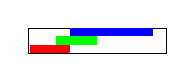
\begin{tikzpicture}[x=5em, y=0.9em]
    \draw [use as bounding box] (0,0) rectangle (1,1);
    \fill [fill=red]   (0.01, 0.01) rectangle (0.3, 0.34);
    \fill [fill=green] (0.2,  0.34) rectangle (0.5, 0.67);
    \fill [fill=blue]  (0.3,  0.67) rectangle (0.9, 0.99);
    \end{tikzpicture}
    \hspace{-0.6em}
}
\def\splitExampleNoncontinuous{
    \hspace{-0.6em}
    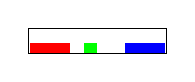
\begin{tikzpicture}[x=5em, y=0.9em]
    \draw [use as bounding box] (0,0) rectangle (1,1);
    \fill [fill=red]   (0.01, 0.01) rectangle (0.3,  0.4);
    \fill [fill=green] (0.4,  0.01) rectangle (0.5,  0.4);
    \fill [fill=blue]  (0.7,  0.01) rectangle (0.99, 0.4);
    \end{tikzpicture}
    \hspace{-0.6em}
}

%% Specify thesis parameters here
%% ----------------------------------------------------------------
\setboolean  {proposal}{false} % disables all stuff that is not needed for a proposal if set to true
\university  {Saarland University}{http://www.uni-saarland.de/}
\department  {Department of Language Science and Technology}{https://www.uni-saarland.de/en/department/lst.html}
\group       {Language Science and 
Technology}{http://www.st.cs.uni-saarland.de/}
\faculty     {Faculty of Arts}{https://www.uni-saarland.de/en/faculty/p/studienangebot-der-philosophischen-fakultaet.html}
\supervisor  {Dietrich Klakow (UdS), Gosse Bouma (RUG),\\Marius Mosbach (UdS, advisor)}
% \advisor     {Your Advisor}
%\examiner    {Who will be grading your thesis}
%\secondexaminer {The second person grading your thesis}
\degree      {Master of Science}
\thesiskind  {Master Thesis}
\authors     {Vilém Zouhar}
\thesistitle {Shrinking Knowledge Base Size:\\ Dimension Reduction, Splitting \& Filtering}
\date        {April 19, 2022}
%\subject     {}
%\keywords    {}
%% ----------------------------------------------------------------

% If this is a proposal prepend 'Proposal for a' to thesiskind
\doifproposal{
	\let\thesisnameproposal\thesisname
	\thesiskind{Report for a \thesisnameproposal}
}

% Enable git revision parsing (Note: you need to enable shell-excape and pipe support for this feature to work)
%\revision{\input{|"git rev-parse HEAD | cut -c 1-8"}}

\begin{document}

\frontmatter	  % Begin Roman style (i, ii, iii, iv...) page numbering

%% Title Page
%% ----------------------------------------------------------------
\maketitle

%% Declaration Page required for the Thesis, your institution may give you a different text to place here
%% ----------------------------------------------------------------
\doifnotproposal{
\begin{declaration}
  \begin{center}
    \bf \large
    Eidesstattliche Erkl\"{a}rung
  \end{center}
  Ich erkl\"{a}re hiermit an Eides Statt,
  dass ich die vorliegende Arbeit selbstst\"{a}ndig verfasst und keine
  anderen als die angegebenen Quellen und Hilfsmittel verwendet habe.
    Ich versichere, dass die gedruckte und die elektronische Version der Masterarbeit inhaltlich übereinstimmen.

  \begin{center}
    \bf \large
    Statement in Lieu of an Oath
  \end{center}
  I hereby confirm that I have written this thesis on my own and 
  that I have not used any other media or materials than the ones
  referred to in this thesis.
  I assure that the electronic version is identical in content to the printed version of the Master's thesis.

%   \vfill
%   \begin{center}
%     \bf \large
%     Einverst\"{a}ndniserkl\"{a}rung
%   \end{center}
%   Ich bin damit einverstanden, dass meine (bestandene) Arbeit in beiden 
%   Versionen in die Bibliothek der Informatik aufgenommen und damit 
%   ver\"{o}ffentlicht wird. 

%   \begin{center}
%     \bf \large
%     Declaration of Consent
%   \end{center}
%   I agree to make both versions of my thesis (with a passing grade) 
%   accessible to the public by having them added to the library of the
%   Computer Science Department.

  \vfill
  \vfill
   
  Datum/Date:\\
  \rule[1em]{25em}{0.5pt}  % This prints a line to write the date

  Unterschrift/Signature:\\
  \rule[1em]{25em}{0.5pt}  % This prints a line for the signature
   
\end{declaration}
  \cleardoublepage  % Declaration ended, now start a new page
}

%% The Abstract Page
%% ----------------------------------------------------------------
\begin{abstract}
	\input{\chapterpath abstract.tex}
\end{abstract}

\doifnotproposal{

%% The Acknowledgements page, for thanking everyone
%% ----------------------------------------------------------------
\begin{acknowledgements}

During my studies I was generously supported financially and non-financially by the Erasmus Mundus European Masters Program in Language and Communication Technologies.
Thank you to the administrators, Bobbye Pernice, Jürgen Trouvain and Ivana Krujiff-Korbayová.

Thanks to everyone who helped in reviewing this thesis, among others Luuk Suurmeijer (HHU), Rishu Kumar (CUNI), Mrinmaya Sachan (ETHz), Ryan Cotterell (ETHz) and Jakub Zavrel.

A part of this work was also funded by the Deutsche Forschungsgemeinschaft (DFG, German Research Foundation) - Project-ID 232722074 - SFB 1102.

\end{acknowledgements}
\cleardoublepage
}

%% Table of Contents
%% ----------------------------------------------------------------

\tableofcontents
\clearpage

%% The Dedication page
%% ----------------------------------------------------------------
% \doifnotproposal{
%   \thispagestyle{empty}  % Page style needs to be empty for this page
%   \dedicatory{Dedicated to WHATEVER.}
% }

\mainmatter	  % Begin normal, numeric (1,2,3...) page numbering

%% Chapters
%% ----------------------------------------------------------------
% Include the chapters of the thesis, as separate files (careful of case-sensitivity and spaces in filenames)
% Capitalized chaptertitles generally look better

\loadchapter{introduction}{Introduction}
\loadchapter{splitting_filtering}{Splitting \& Filtering}
\loadchapter{dim_reduction}{Dimension Reduction}
\loadchapter{discussion}{Discussion}

\clearpage

%% Appendices
%% ----------------------------------------------------------------
\appendix
% \beginappendix %Begins the appendix

\loadappendix{fusion_discussion}{Fusion Discussion}

\backmatter

%% Lists of figures and tables
%% ----------------------------------------------------------------
\doifnotproposal{
	\lhead{\emph{List of Figures}}
	\addtotoc{List of Figures}
	\listoffigures
	\clearpage

  	\addtotoc{List of Tables}
  	\lhead{\emph{List of Tables}}
	\listoftables
	\clearpage
}

%% Bibliography
%% ----------------------------------------------------------------
\label{Bibliography}
\addtotoc{Bibliography}
\lhead{\emph{Bibliography}}  % Change the left side page header to "Bibliography"
\bibliographystyle{unsrtnat}  % Use the "unsrtnat" BibTeX style for formatting the Bibliography
\bibliography{misc/bibliography.bib}  % The references (bibliography) information are stored in the file named "Bibliography.bib"

% \loadappendix{appendix}{Dimension Reduction}
\end{document}  % The End
